\section{Wavelet disturbance shedding demonstration}
\label{app:wavelet-disturbance-demonstration}

This demonstration run illustrates boundary accounting after the ontology has been declared. It uses one wavelet group on one retained field and records lead--lag span, PADAR burden, shed excess, outward shedding, local reclosure, and reclosure-path triggers.

\paragraph{Demonstration state.}
For tick \(t\), let \(L_t\) be the lead component, \(G_t\) the lag component, \(S_t\) the disturbance span, \(P_t\) the PADAR burden, \(C_t\) local closure compatibility, \(X_t\) shed excess, \(O_t\) outward shedding, and \(R_t\) local reclosure:
\[
S_t=|L_t-G_t|,
\qquad
\widetilde P_t=\eta_{\mathrm{ret}} P_{t-1}+\gamma_{\mathrm{span}} S_t,
\]
\[
X_t=\max(0,\widetilde P_t-C_t),
\qquad
P_t=\widetilde P_t-X_t,
\]
\[
O_t=(1-\lambda_{\mathrm{reclose}})X_t,
\qquad
R_t=\lambda_{\mathrm{reclose}}X_t.
\]
A reclosure-path trigger is recorded when \(R_t\) crosses the declared local reclosure threshold.

\paragraph{Displayed run.}
The displayed run uses \(90\) ticks, retention coefficient \(\eta_{\mathrm{ret}}=0.82\), span gain \(\gamma_{\mathrm{span}}=0.55\), and reclosure fraction \(\lambda_{\mathrm{reclose}}=0.38\). The lead and lag components are declared deterministic test streams with two local disturbance pulses. The run demonstrates the accounting pattern for shed disturbance and local reclosure.

\begin{figure}[H]
\centering
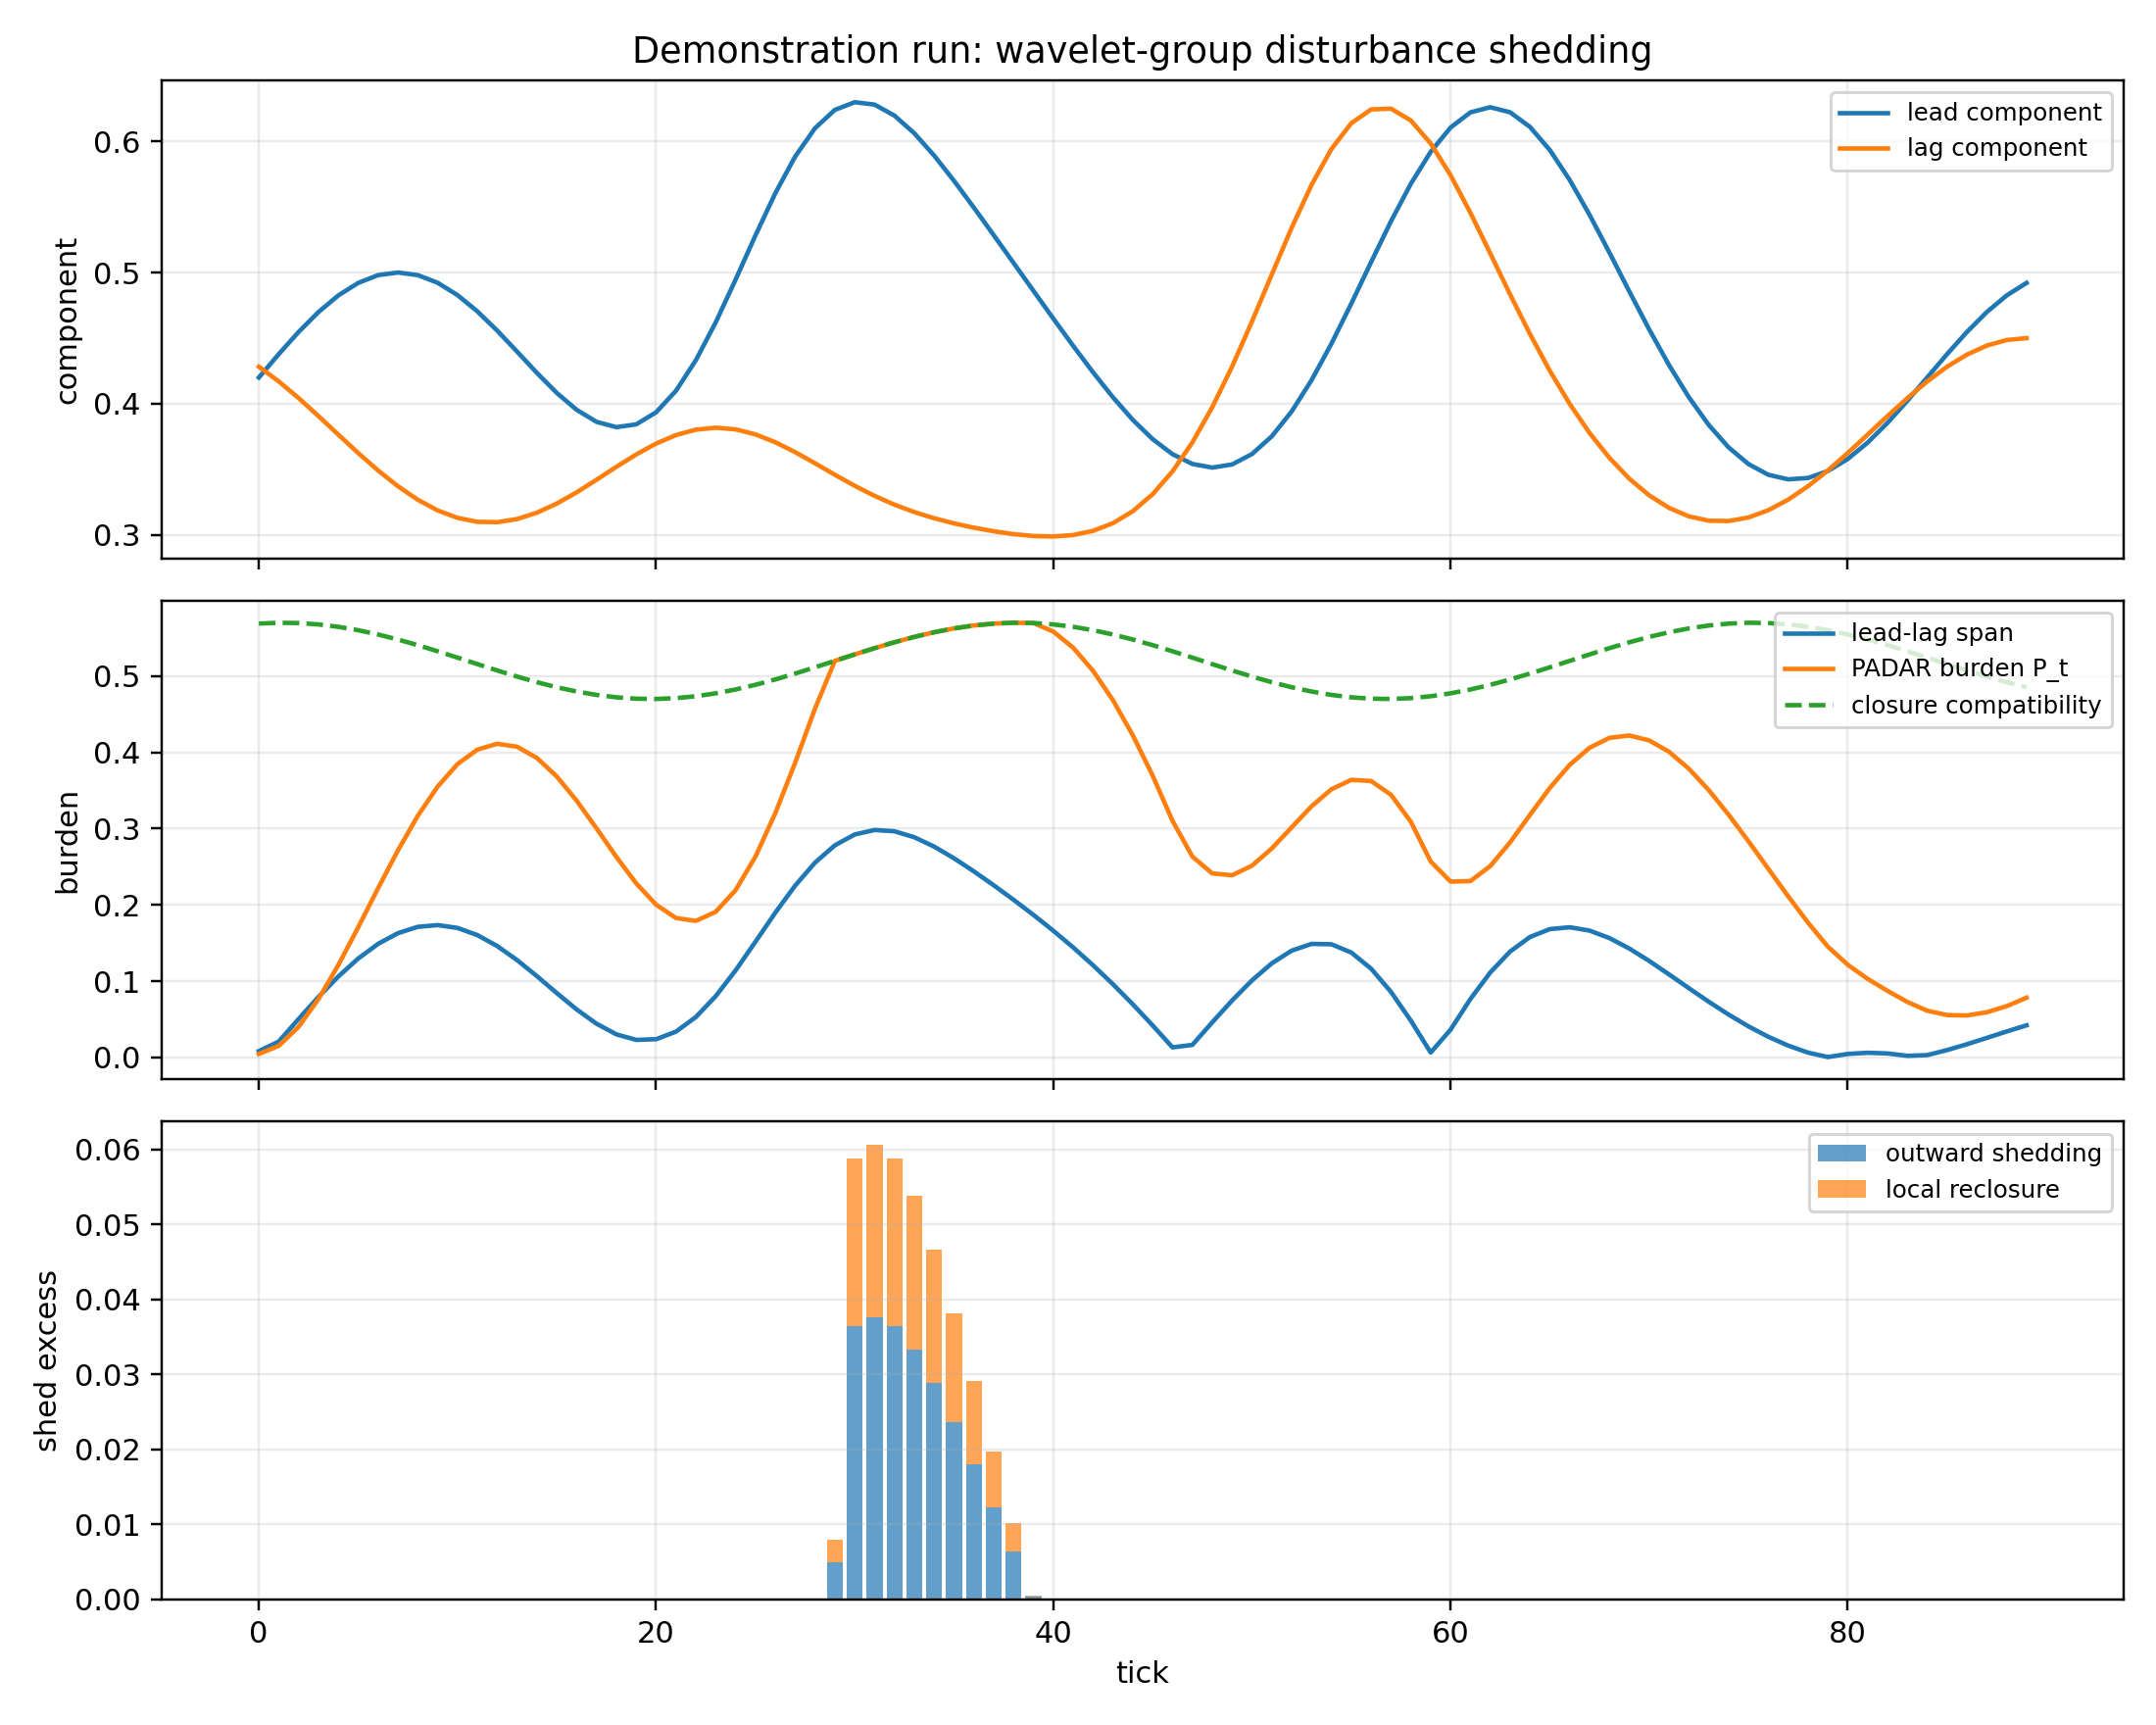
\includegraphics[width=0.98\linewidth]{figures_jpg/v39_wavelet_disturbance_shedding_simulation.png}
\caption{Demonstration run: wavelet-group disturbance shedding. The upper panel shows lead and lag components. The middle panel shows disturbance span, PADAR burden, and local closure compatibility. The lower panel shows outward shedding, local reclosure, and the reclosure-path trigger.}
\label{fig:v39-wavelet-shedding-simulation}
\end{figure}

\paragraph{Run summary.}
\begin{center}
\begin{tabular}{lr}
\toprule
Update steps & 90 \\
Maximum lead-lag span & 0.298 \\
Maximum PADAR burden & 0.570 \\
Maximum shed excess & 0.061 \\
Total outward shedding & 0.238 \\
Total local reclosure & 0.146 \\
Shell-reclosure trigger updates & 0 \\
First reclosure update & none \\
\bottomrule
\end{tabular}

\end{center}
